\subsection{Question 1}

\lstinputlisting[caption=Matlab Commands,showstringspaces=false,language=Matlab]{../find_vectors.m}

\newpage
\subsubsection{Part A}

\lstinputlisting[caption=Matlab Commands,showstringspaces=false,language=Matlab]{../q1_partA}

\subsubsection{Part B}

\lstinputlisting[caption=Matlab Commands,showstringspaces=false,language=Matlab]{../q1_partB}

\newpage
\subsection{Question 2}

\begin{figure}[th]
  \centering
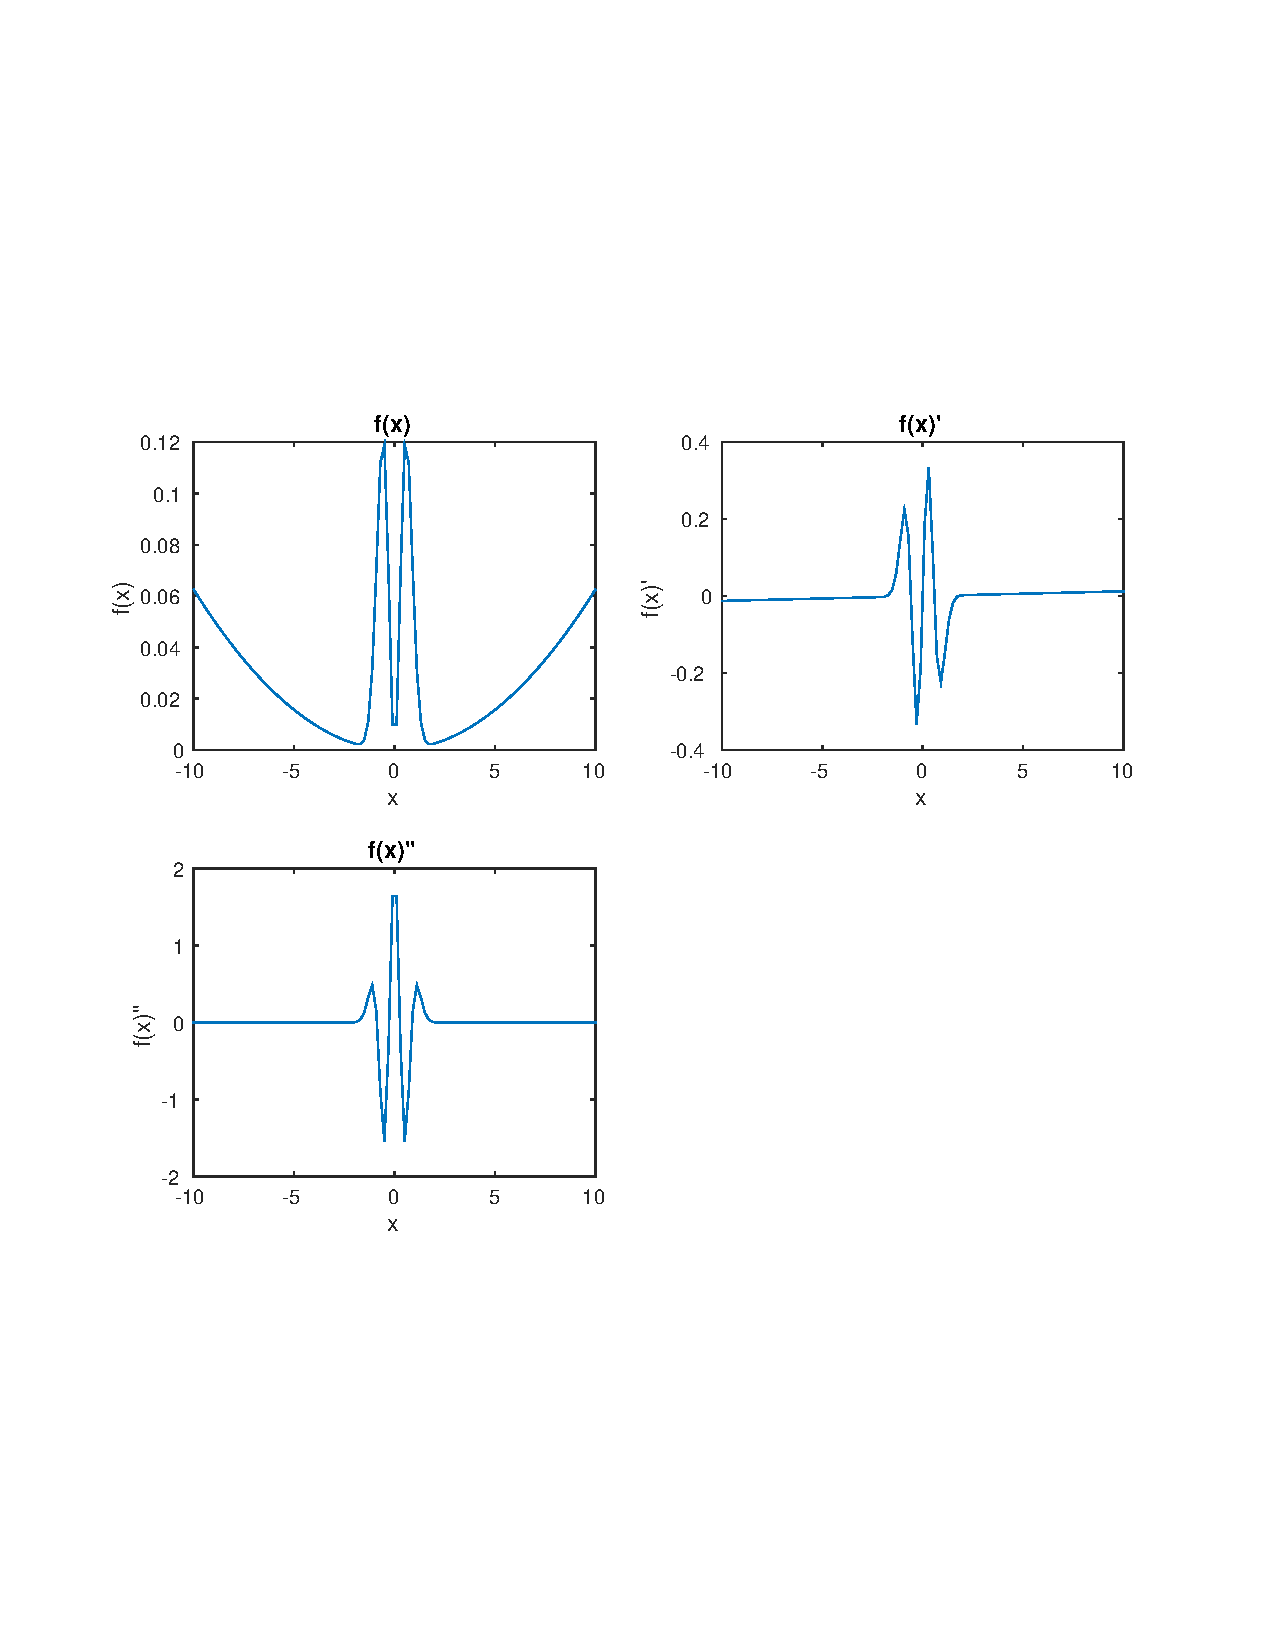
\includegraphics[trim=10mm 70mm 10mm 70mm, width=1.0\textwidth]{../q2_plots}
\end{figure}

\lstinputlisting[caption=Matlab Commands,showstringspaces=false,language=Matlab]{../q2_maxmin}

\newpage
\lstinputlisting[caption=Matlab Commands,showstringspaces=false,language=Matlab]{../q2_plots}

\newpage
\subsection{Question 3}

\subsubsection{Part C}

The claim made from assignment 2 question 3 part B was as follows:

\begin{eqnarray}
  ||A^{-1}||_2 = \max_{s_A \in s(A)} \{\frac{1}{s_a}\}
\end{eqnarray}

We must find a formula for the condition number of \(A\), \(c_2(A)\), in terms of \(\sigma(A'A)\).
Note, we know \(||A||_2 = \max \{ s(A) \}\) where \(s(A)\) are the singular values of \(A\).
The formula for the condition number of \(A\) is as follows:

\begin{eqnarray}
  c_2(A) = ||A||_2||A^{-1}||_2
  \label{form:c2}
\end{eqnarray}

Therefore, to define \(c_2(A)\) in terms of the \(\sigma(A'A)\) we simply substitute our formulas for \(||A||_2\) and \(||A^{-1}||_2\) into (\ref{form:c2}).
This yeilds,

\begin{eqnarray}
  c_2(A) = \max \{s(A)\} \max_{s_A \in s(A)} \{\frac{1}{s_a}\}
\end{eqnarray}

\subsubsection{Part D}

The claim made from assignment 2 question 2 part E was as follows:

\begin{eqnarray}
  s(A) = \{|\lambda| : \lambda \in \sigma(A), \lambda \neq 0\}
  \label{form:sasym}
\end{eqnarray}

Stated, this says ''The singular values of a matrix \(A\) are the absolute values of the non-zero eigenvalues of \(A\), where \(A\) is symmetric''.

The formula for the condition number of a symmetric matrix \(A\) is the same as the formula stated in part C.
The only change in definition is that of the singular values of \(A\).
Thefore the formula, using the definition of \(s(A)\) from \ref{form:sasym}, is,

\begin{eqnarray}
  c_2(A) &=& \max \{s(A)\} \max_{s_A \in s(A)} \{\frac{1}{s_a}\}
\end{eqnarray}

\newpage
\subsubsection{Part E}

\lstinputlisting[caption=Matlab Commands,showstringspaces=false,language=Matlab]{../q3_partE}



\newpage
\subsection{Question 4}

\subsubsection{Part A}

\lstinputlisting[caption=Matlab Commands,showstringspaces=false,language=Matlab]{../q4_partA.m}

\subsubsection{Part B}

\lstinputlisting[caption=Matlab Commands,showstringspaces=false,language=Matlab]{../q4_partB.m}

\newpage
\subsubsection{Part C}

\begin{figure}[th]
  \centering
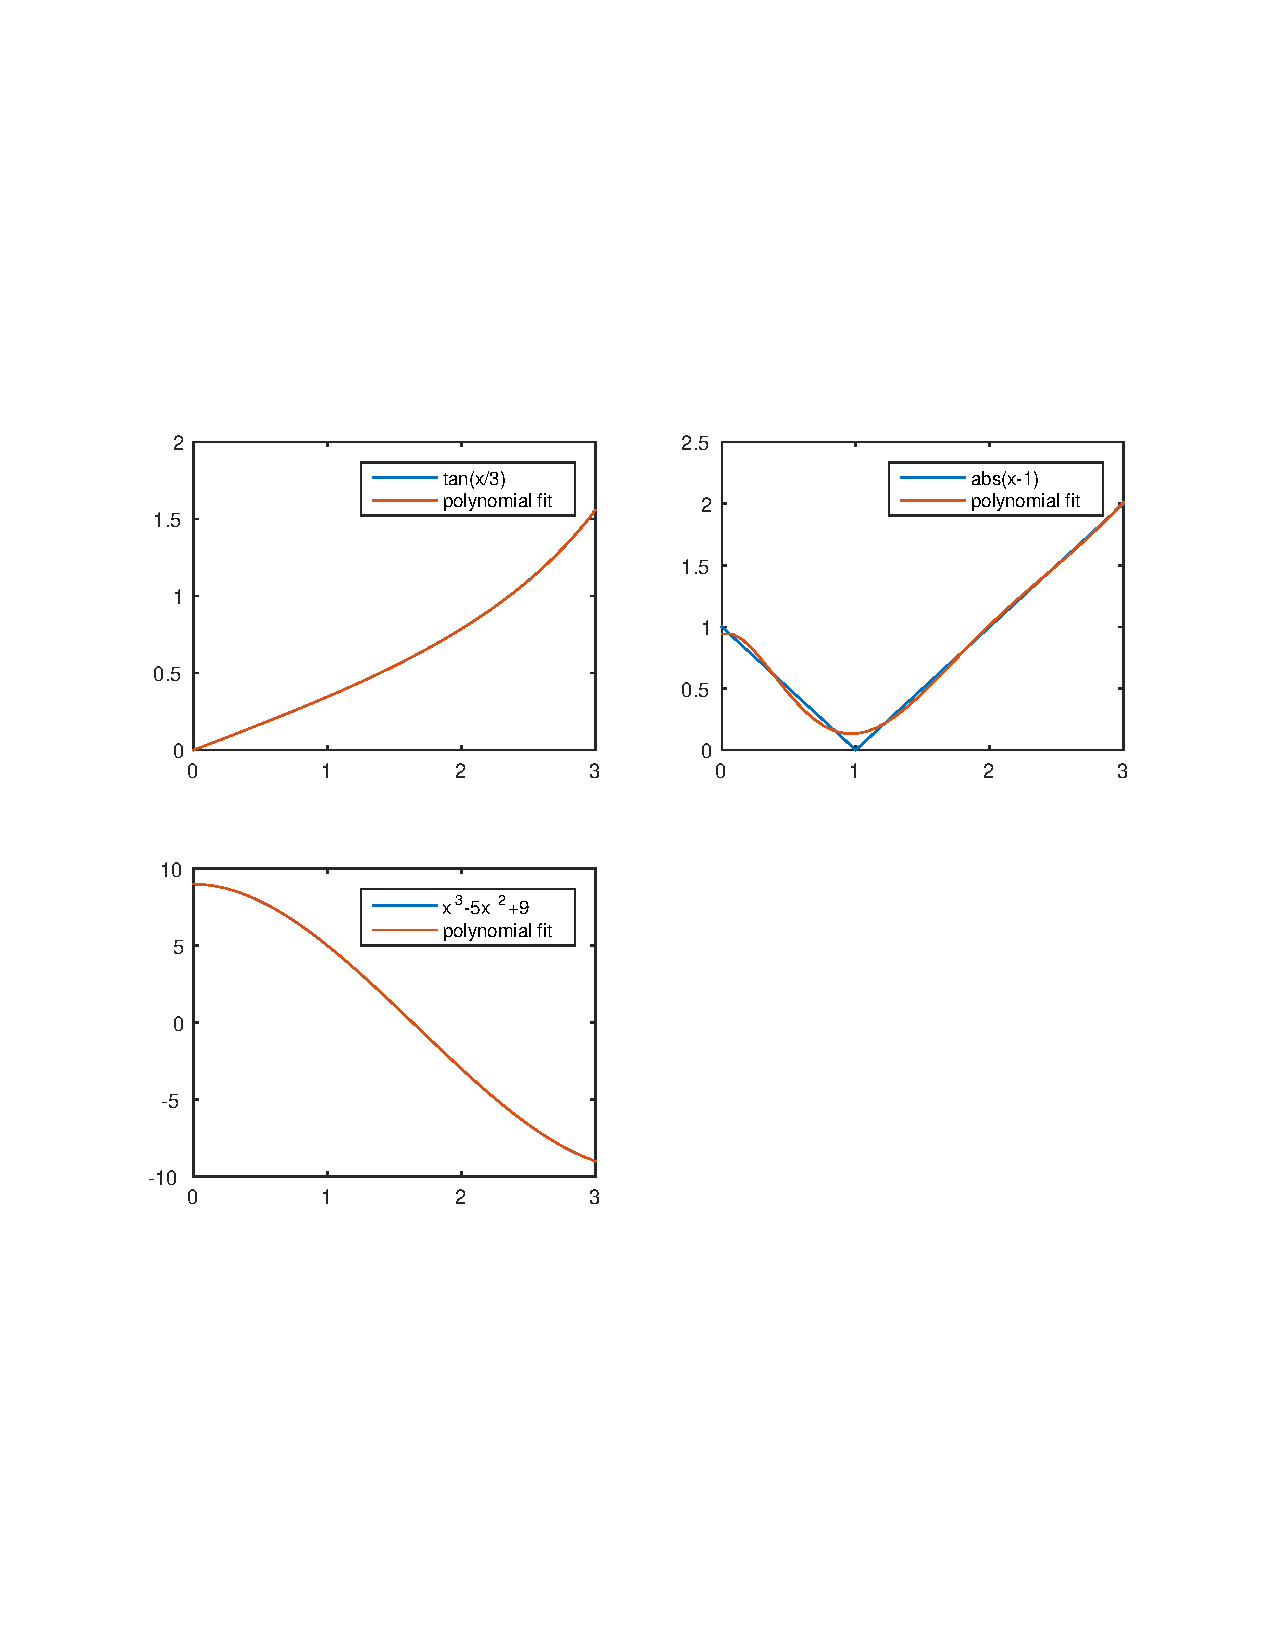
\includegraphics[trim=10mm 70mm 10mm 70mm, width=1.0\textwidth]{../q4_plots}
\end{figure}

From these plots we can see that a higher order polynomial is quite good at fitting a lower order polynomial on a small range.
This is apparent from the plots of \(\tan(\frac{x}{3})\) and \(x^{3}-5x^{2}+9\).
However, the fit is less tight for \(|x-1|\), a function that has a point where it is not differentiable (e.g., in general, non-smooth functions).

\newpage
\lstinputlisting[caption=Matlab Commands,showstringspaces=false,language=Matlab]{../q4_partC}

\newpage
\subsection{Question 5}
\subsubsection{Part A}

We must prove that a matrix \(A\) with a real Cholesky factorization is symmetric positive definite.
Therefore we must prove two things.
The first is that \(A\) is positive definite.
The second is that \(A\) is symmetric.
To this end we know \(A = C'C\).

Therefore we can prove positive definiteness simply as follows,

\begin{eqnarray}
  (Av,v) &\ge& 0 \\
  (C'Cv,v) &\ge& 0 \\
  (Cv,Cv) &\ge& 0
\end{eqnarray}

This concludes the proof for positive definiteness.

Next, we will prove that \(A\) is symmetric.
Note, a matrix \(A\) is symmetric if \(A = A'\).
The proof is a simple substitution as follows,

\begin{eqnarray}
  A &=& A' \\
  C'C &=& (C'C)' \\
  C'C &=& C'C
\end{eqnarray}

This concludes the proof that \(A\) is symmetric.
The proof that \(A\) is symmetric positive definite is complete.

\subsubsection{Part B}
\subsubsection{Part C}
\subsubsection{Part D}

\newpage
\subsection{Question 6}

%\lstinputlisting[caption=Matlab Commands,showstringspaces=false,language=Matlab]{../q5_partC}
